\documentclass[border=5pt]{standalone}
\usepackage[T1]{fontenc}
\RequirePackage[semibold]{sourcesanspro}
\usepackage{pgfplots}
\usepackage{xcolor}
\usetikzlibrary{patterns}

\pgfplotsset{compat=1.18}

% Define colors
\definecolor{hyalinesolid}{HTML}{2171B5}
\definecolor{hyalinehatch}{HTML}{A6C8E8}
\definecolor{esmsolid}{HTML}{E8833A}
\definecolor{esmhatch}{HTML}{F4C9A8}
\definecolor{randomsolid}{HTML}{707070}
\definecolor{randomhatch}{HTML}{C0C0C0}
\definecolor{textgray}{HTML}{404040}
\definecolor{gridgray}{HTML}{E0E0E0}

\begin{document}
\sffamily
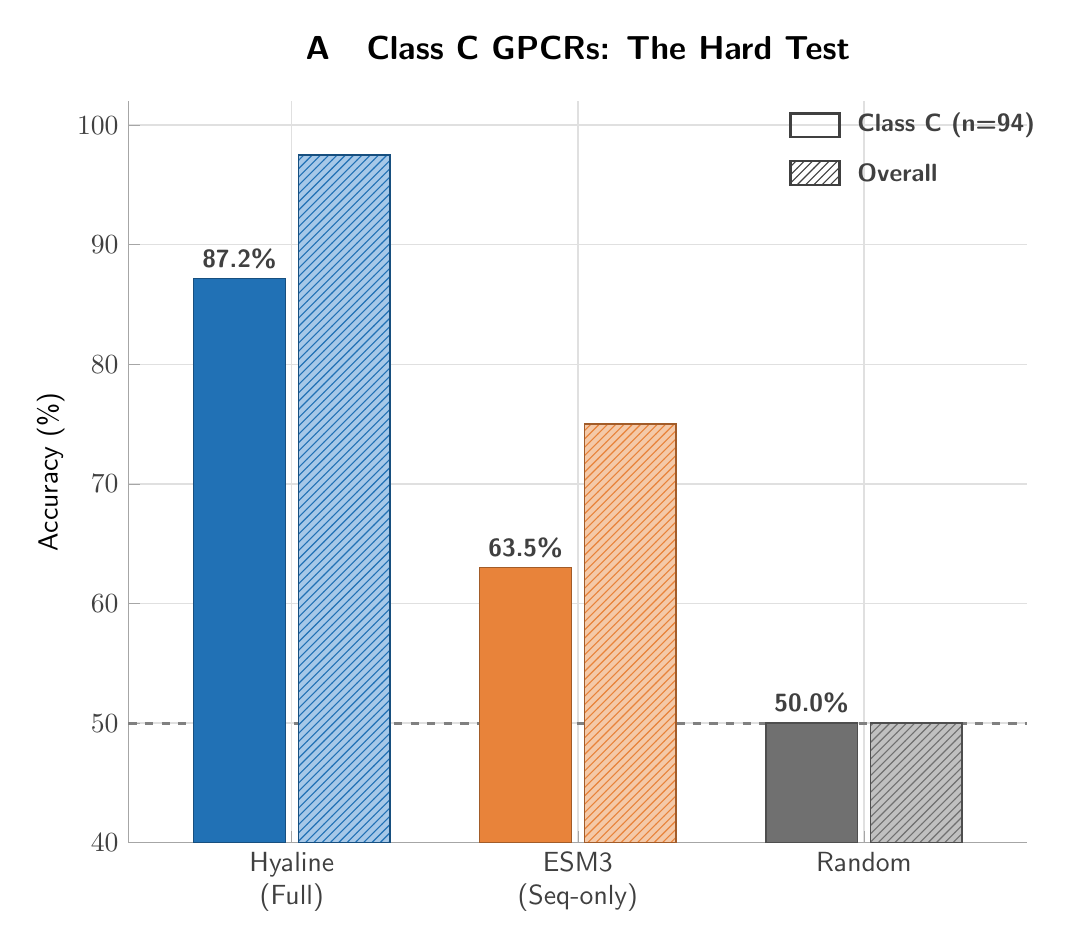
\begin{tikzpicture}

\begin{axis}[
    font=\footnotesize\sffamily,
    width=13cm,
    height=11cm,
    ymin=40,
    ymax=102,
    xmin=0,
    xmax=5.5,
    xtick={1, 2.75, 4.5},
    xticklabels={Hyaline\\(Full), ESM3\\(Seq-only), Random},
    xticklabel style={font=\normalsize\sffamily, color=textgray, align=center},
    ytick={40, 50, 60, 70, 80, 90, 100},
    yticklabel style={font=\normalsize\sffamily, color=textgray},
    ylabel={Accuracy (\%)},
    ylabel style={font=\normalsize\sffamily, at={(-0.06,0.5)}},
    title={\textbf{A\quad Class C GPCRs: The Hard Test}},
    title style={font=\large\sffamily\bfseries, at={(0.5,1.02)}},
    axis line style={gray!70, line width=0.5pt},
    tick style={gray!70},
    ymajorgrids=true,
    xmajorgrids=true,
    grid style={gridgray, line width=0.5pt},
    axis x line*=bottom,
    axis y line*=left,
    clip=false,
]

% Bar width and offset for paired bars
\pgfmathsetmacro{\barwidth}{0.28}
\pgfmathsetmacro{\offset}{0.32}

% Dashed line at 50%
\draw[gray, dashed, line width=1.2pt] (axis cs:0,50) -- (axis cs:5.5,50);

% === Hyaline (Full) - centered at x=1 ===
% Class C (solid blue)
\fill[hyalinesolid] (axis cs:1-\offset-\barwidth,40) rectangle (axis cs:1-\offset+\barwidth,87.2);
\draw[hyalinesolid!70!black, line width=0.5pt] (axis cs:1-\offset-\barwidth,40) rectangle (axis cs:1-\offset+\barwidth,87.2);
\node[font=\small\sffamily\bfseries, color=textgray, above] at (axis cs:1-\offset,87.2) {87.2\%};

% Overall (hatched blue)
\fill[hyalinehatch] (axis cs:1+\offset-\barwidth,40) rectangle (axis cs:1+\offset+\barwidth,97.5);
\draw[pattern=north east lines, pattern color=hyalinesolid] (axis cs:1+\offset-\barwidth,40) rectangle (axis cs:1+\offset+\barwidth,97.5);
\draw[hyalinesolid!70!black, line width=0.5pt] (axis cs:1+\offset-\barwidth,40) rectangle (axis cs:1+\offset+\barwidth,97.5);

% === ESM3 (Seq-only) - centered at x=2.75 ===
% Class C (solid orange)
\fill[esmsolid] (axis cs:2.75-\offset-\barwidth,40) rectangle (axis cs:2.75-\offset+\barwidth,63);
\draw[esmsolid!70!black, line width=0.5pt] (axis cs:2.75-\offset-\barwidth,40) rectangle (axis cs:2.75-\offset+\barwidth,63);
\node[font=\small\sffamily\bfseries, color=textgray, above] at (axis cs:2.75-\offset,63) {63.5\%};

% Overall (hatched orange)
\fill[esmhatch] (axis cs:2.75+\offset-\barwidth,40) rectangle (axis cs:2.75+\offset+\barwidth,75);
\draw[pattern=north east lines, pattern color=esmsolid] (axis cs:2.75+\offset-\barwidth,40) rectangle (axis cs:2.75+\offset+\barwidth,75);
\draw[esmsolid!70!black, line width=0.5pt] (axis cs:2.75+\offset-\barwidth,40) rectangle (axis cs:2.75+\offset+\barwidth,75);

% === Random - centered at x=4.5 ===
% Class C (solid gray)
\fill[randomsolid] (axis cs:4.5-\offset-\barwidth,40) rectangle (axis cs:4.5-\offset+\barwidth,50);
\draw[randomsolid!70!black, line width=0.5pt] (axis cs:4.5-\offset-\barwidth,40) rectangle (axis cs:4.5-\offset+\barwidth,50);
\node[font=\small\sffamily\bfseries, color=textgray, above] at (axis cs:4.5-\offset,50) {50.0\%};

% Overall (hatched gray)
\fill[randomhatch] (axis cs:4.5+\offset-\barwidth,40) rectangle (axis cs:4.5+\offset+\barwidth,50);
\draw[pattern=north east lines, pattern color=randomsolid] (axis cs:4.5+\offset-\barwidth,40) rectangle (axis cs:4.5+\offset+\barwidth,50);
\draw[randomsolid!70!black, line width=0.5pt] (axis cs:4.5+\offset-\barwidth,40) rectangle (axis cs:4.5+\offset+\barwidth,50);

% === Generic Legend (top right) ===
% Solid bar entry (outline only, white fill)
\fill[white, fill opacity=0] (axis cs:4.05,99) rectangle (axis cs:4.35,101);
\draw[textgray, line width=1pt] (axis cs:4.05,99) rectangle (axis cs:4.35,101);
\node[anchor=west, font=\small\sffamily\bfseries, color=textgray] at (axis cs:4.4,100) {Class C (n=94)};

% Hatched bar entry
\fill[white] (axis cs:4.05,95) rectangle (axis cs:4.35,97);
\draw[pattern=north east lines, pattern color=textgray] (axis cs:4.05,95) rectangle (axis cs:4.35,97);
\draw[textgray, line width=1pt] (axis cs:4.05,95) rectangle (axis cs:4.35,97);
\node[anchor=west, font=\small\sffamily\bfseries, color=textgray] at (axis cs:4.4,96) {Overall};

\end{axis}

\end{tikzpicture}
\end{document}